\chapter{Spin Analysis}
\label{ch:spin_analysis}
\section{Introduction}

The overall goal of this analysis is to calculate the longitudinal asymmetry,
$A_L$, for $W\rightarrow\mu$ production. As discussed in
Chapter~\ref{ch:modeling_proton_spin}, $A_L$ is an important probe for the
polarized parton distribution functions describing the quarks and anti-quarks of
the proton sea-quark population. $A_L$ provides an excellent probe in the case
of the $W$ interaction because of the parity violating nature of the
interaction. The $W^+$ interacts only with left handed quarks and right-handed
anti-quarks, with respect to sea-quark interaction. This means that measurement
of the $W^+$ asymmetry gives direct access to the initial helicity state of $u$
and $\bar{d}$, while $W^-$ gives direct access to $d$ and $\bar{u}$, and even
then, the interaction is only permitted providing that either of the quarks are
in an allowed initial helicity state.

{\noindent}$A_L$ can be written in terms of experimental yields for a process,
or in terms of the scattering amplitudes of the $W\rightarrow\mu$ process:

\begin{enumerate}
  \item Write it in terms of the machine luminosity and the number of events of
    a particular type observed
  \item Calculate the scattering amplitude for the process, and then the
    cross-section of the process. Write down the cross-section in terms of
    experimental observables.
\end{enumerate}

Global fits have been carried by the DSSV analysis group~\cite{DeFlorian2009}
which predict the helicity distribution of various partons in the proton. These
fits suffer from large uncertainties, which may be reduced via measurement of
the asymmetry.

One measures this asymmetry, as discussed in item (1), and this measurement is
then fed back into the models in order to reduce the degrees of freedom in the
existing model reduce the uncertainty of the models' predictions. 

The remaining task in this analysis, after an understanding of the signal to
background ratio, and a means to estimate the real yields of the $W$ signal
event is to calculate asymmetries.

{\noindent}The Asymmetry Calculation relies on understanding the following items
quantitatively:

\begin{enumerate}
  \item What is the total beam polarization?
  \item What is the polarization of the blue bunch, and yellow bunch at the
    time of each beam-beam interaction which generated a W-genic muon?
  \item What is the total yield of $\mu$'s at forward and backward rapidity,
    for positive and negative charge?
\end{enumerate}

{\noindent}$A_L$ is then calculated:

\begin{equation}
  A_L = {
    {d\sigma^{\Rightarrow} - d\sigma^{\Leftarrow}}
    \over
    {d\sigma^{\Rightarrow} + d\sigma^{\Leftarrow}}
  }
\end{equation}

{\noindent}Where $d\sigma$ is calculated as:

\begin{equation}
  d\sigma = {1\over{\mathcal{L}}}{\dot{N}},
\end{equation}

with $\Rightarrow$ or $\Leftarrow$ referring to tracks which come from
positive($\Rightarrow$) or negative($\Leftarrow$) helicities relative to the
initial proton polarization state. $\mathcal{L}$ refers to the beam luminosity,
a property of the colliding beams, and $\dot{N}$ refers to the production rate
of W-genic muons. This calculation is done for forward and backward
rapidities for positively and negatively charged muons, with associated
asymmetries calculated individually for each arm and charge. The asymmetries are
then summed according to the charge of the parent $W$ boson.

In practice, one does not need to calculate cross-sections for $W\rightarrow\mu$ for
the purposes of evaluating $A_L$. Only yields are needed, since in principal
$\mathcal{L}$ will be a common factor in all cross-sections and cancel out. This
of course comes with major caveats--$\mathcal{L}$ only cancels out if the
relative luminosity of each polarization condition is the same. Spin patterns
are chosen in order to ensure this happens. This is verified by counting the
number of polarization states observed, and ensuring that all states occur with
the same frequency.  Experimentally, raw asymmetries, ($\epsilon_{L}$), are
constructed from  muon yields in the same way as $A_L$ but without correction
for background dilution or beam polarization. With those factors applied, we may
transform the raw asymmetry to the true longitudinal asymmetry. This is further
discussed in Section~\ref{sec:calculating_al}

\section{Measured Beam Polarization}
\label{sec:measured_beam_polarization}

Beam polarization is obtained from the p-Carbon scattering experiments done for
every polarized fill. Because fills are eight hours each, several consecutive
runs in the same fill will share the same spin pattern, but the overall
polarization of the beam may change as a function of time due to depolarizing
resonances. The data archived during these measurements is stored to a database,
and an analysis, `spin database QA', performs consistency checks to ensure that
polarization patterns do not change over the course of a fill, and are
consistent with the advertised polarization pattern. This study also produces
the average beam polarization per run. The polarization of the beams are
measured at the beginning and end of every fill. This was described in
Section~\ref{sec:beam_polarization}. The results of the polarization study and
spin database QA are all stored in a PostgreSQL database, indexed by run number.
The average percent polarization of the blue and yellow beams over the Run 13
run are summarized in Figure~\ref{fig:avg_polarization} and
Figure~\ref{fig:pol_distribution}.

\begin{figure}[ht]
  \centering
  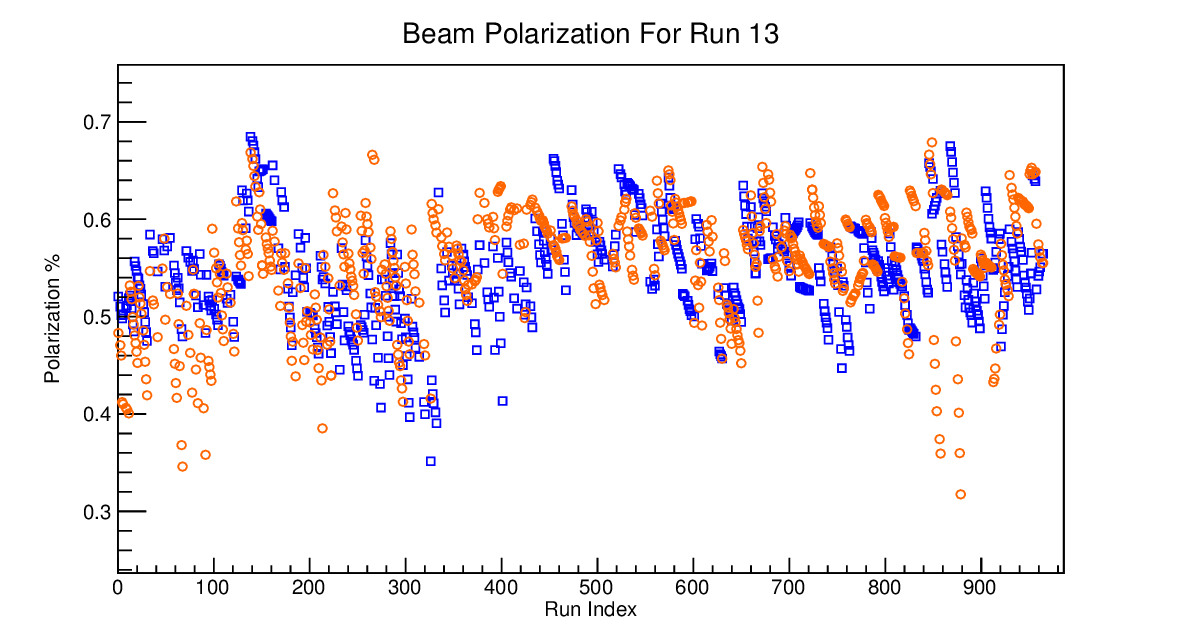
\includegraphics[width=\linewidth]{./figures/beam_polarization.jpg}
  \caption{
    Shown: the average beam polarization per run over the course of the 2013
    data set. All of the runs in the analysis were indexed from 0 to
    approximately 1000, and plotted in the order that they were taken. The blue
    open circles are from the blue beam, the yellow open circles are for the
    yellow beam.
  }
  \label{fig:avg_polarization}
\end{figure}

The average beam polarization over the whole of Run 13 was well over 50\% for
the majority of the run, with a few poorly polarized runs. This is accounted for
by calculating asymmetries for individual runs which are weighted by that run's
average polarization. It was found that the final asymmetry resulting from
individual run weighting was the same using the average polarization for all
runs. This indicates that the polarization for most of the recorded data was
consistent.  The average beam polarization for each run in the Run 13 data set
is summarized in Figure~\ref{fig:avg_polarization}, indicating a consistent,
regular distribution. The average beam polarization is also visualized as a
histogram to highlight the overall distribution of polarizations in the 2013
data set, Figure~\ref{fig:pol_distribution}.

\begin{figure}[H]
	\centering
	\begin{subfigure}[t]{0.5\textwidth}
		\centering
		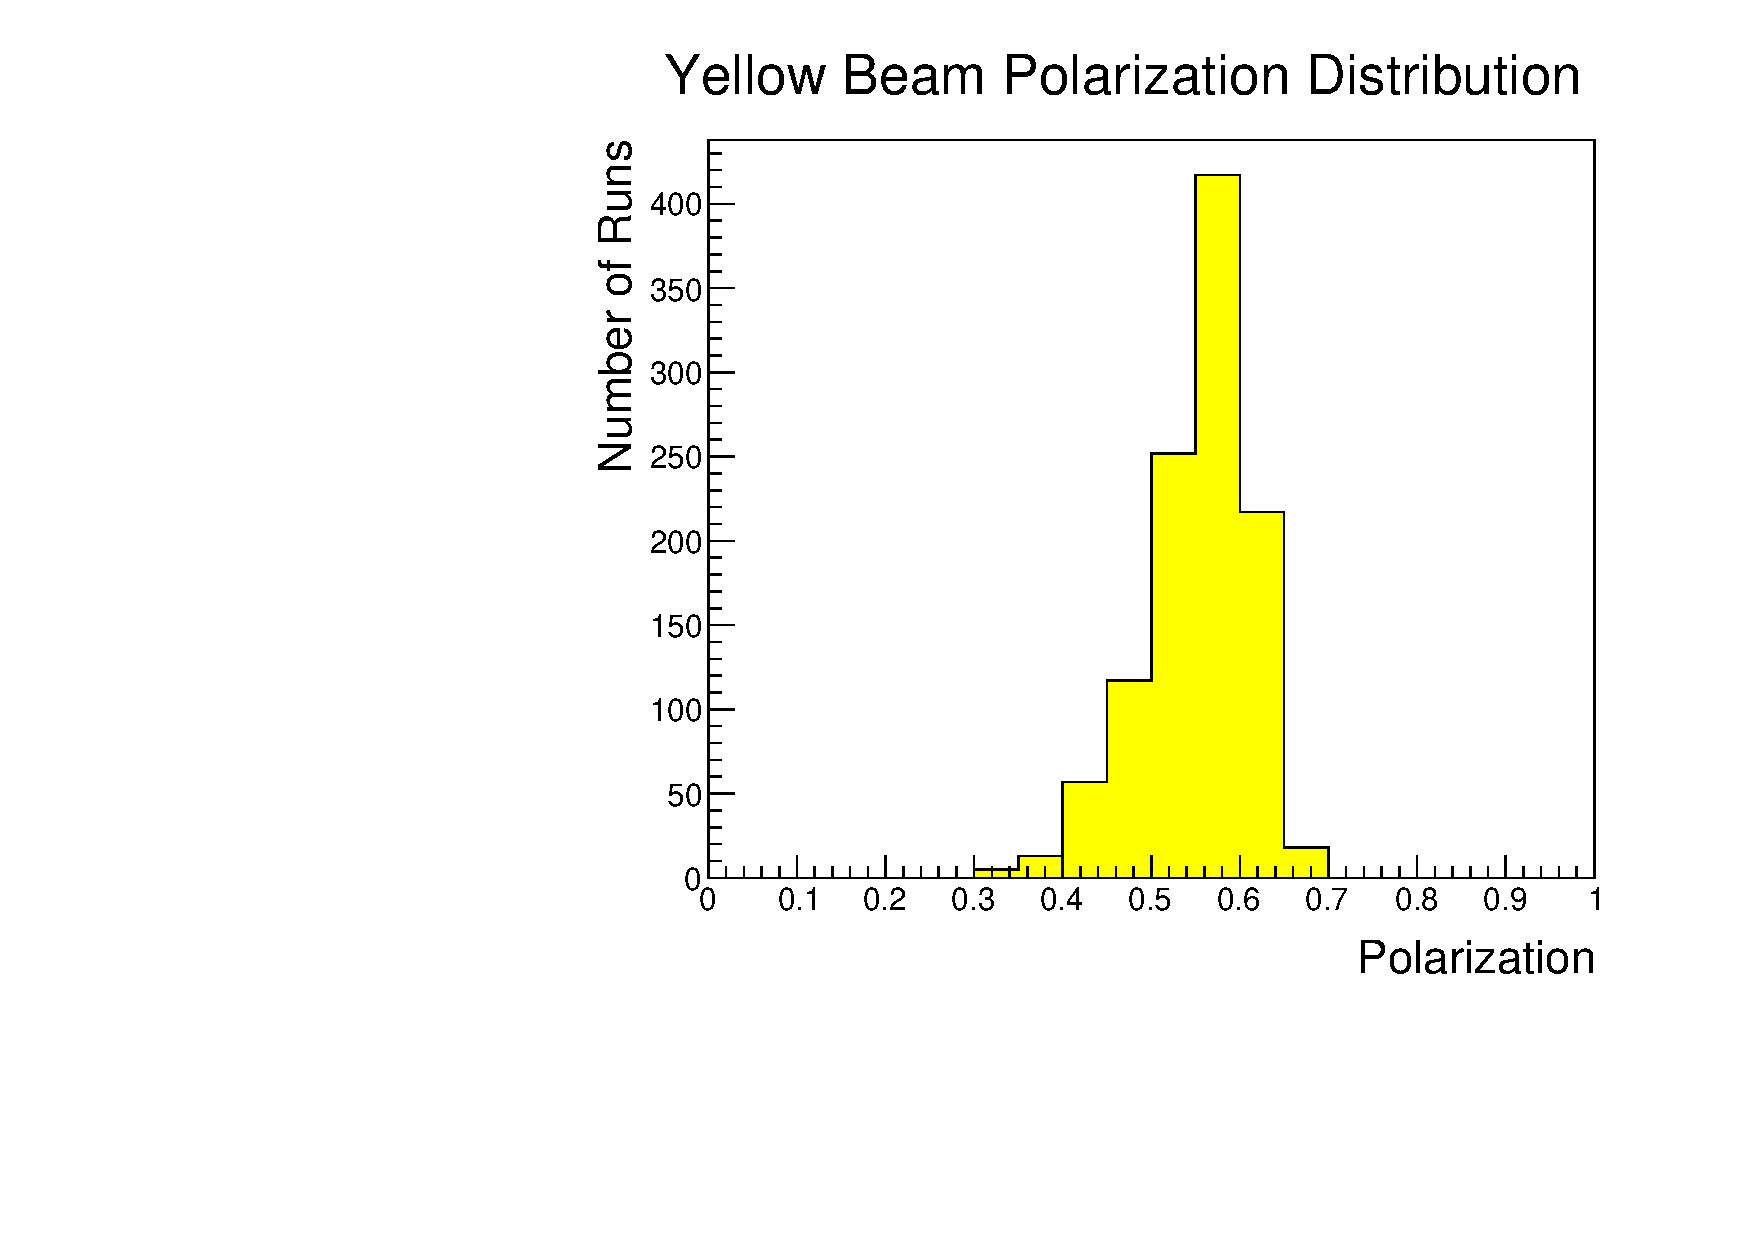
\includegraphics[width=0.95\linewidth]{./figures/yell_polarization.pdf}
		\caption{Distribution of Yellow Beam Polarization}
		\label{fig:pol_yell}
	\end{subfigure}%
  \begin{subfigure}[t]{0.5\textwidth}
		\centering
		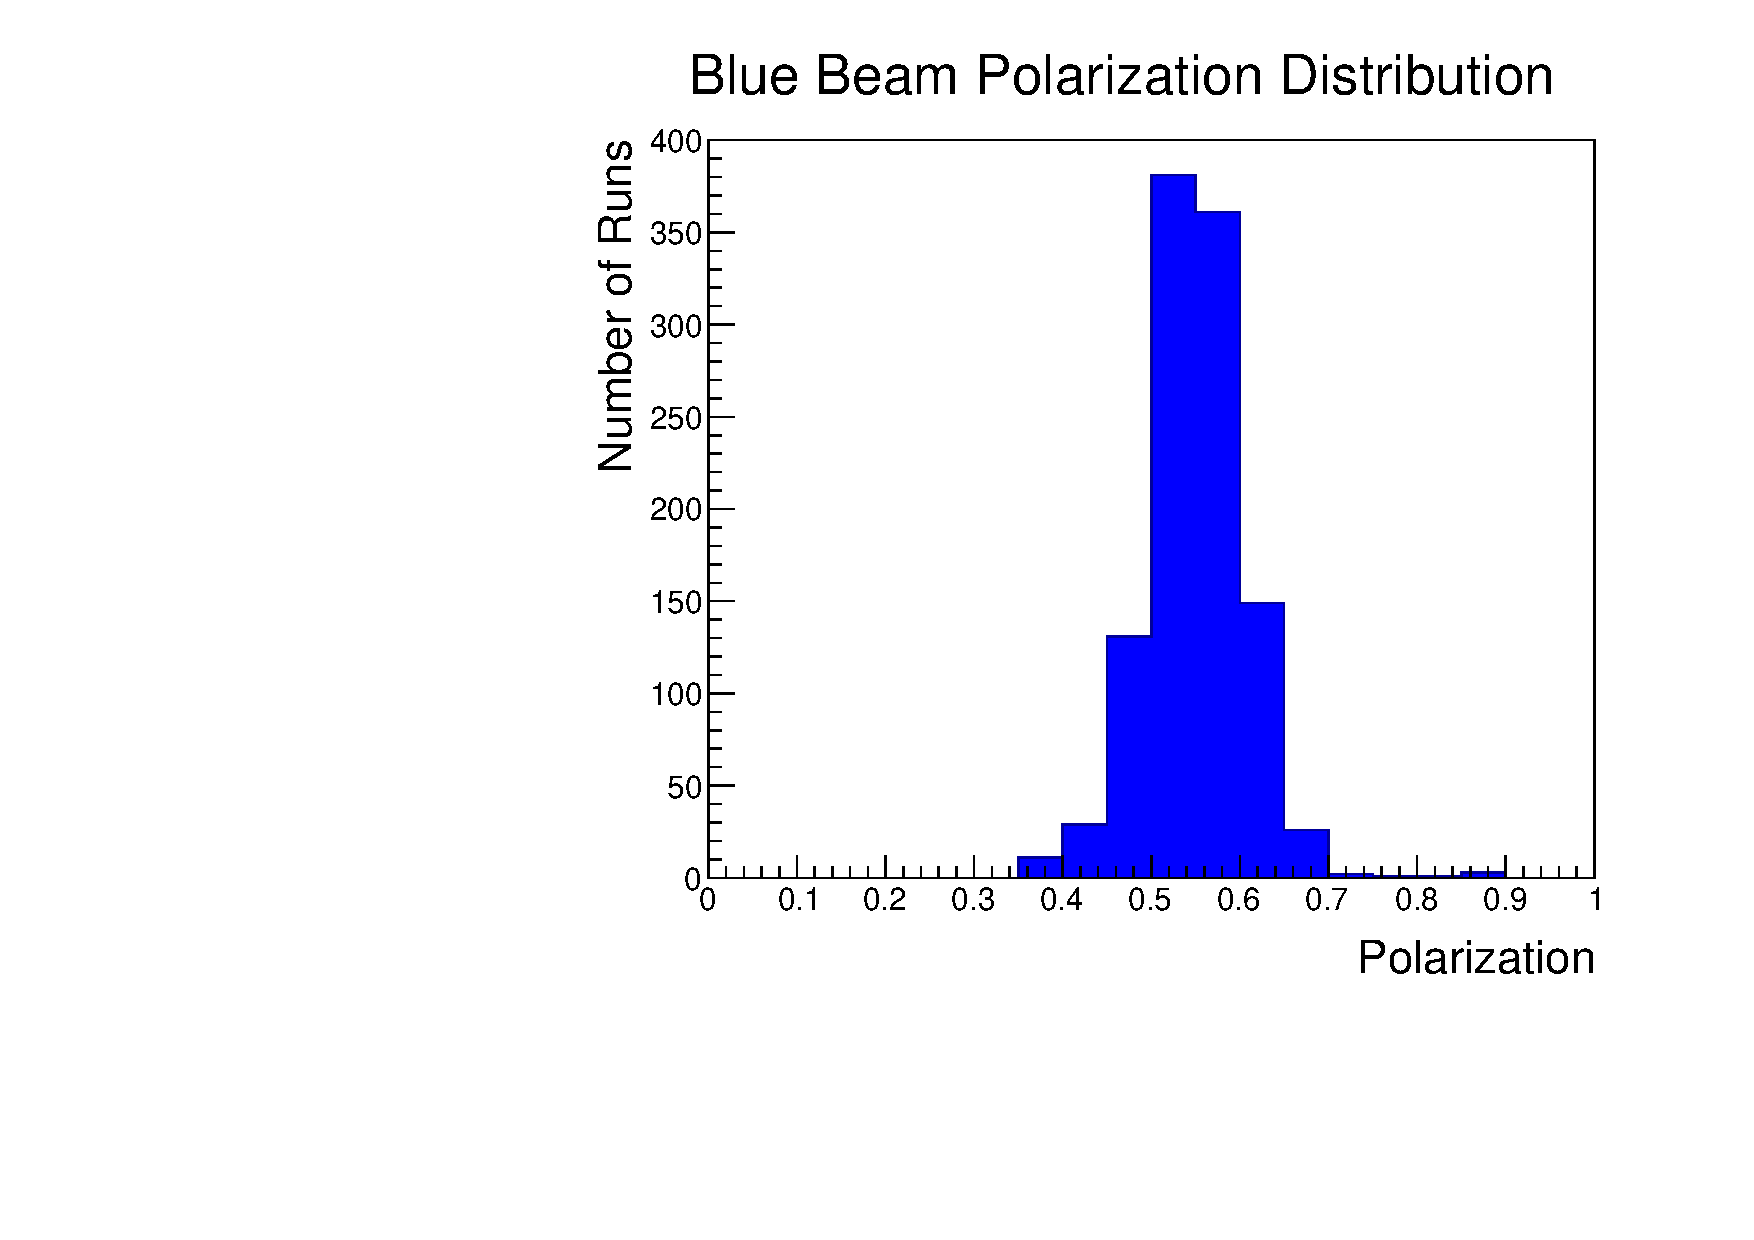
\includegraphics[width=0.95\linewidth]{./figures/blue_polarization.pdf}
    \caption{Distribution of Blue Beam Polarization}
		\label{fig:pol_blue}
	\end{subfigure}
	\caption{ 
    Panel (a) shows the yellow beam polarization distribution over all runs in
    the 2013 data taking period, with an average of about 55.27\%. Panel (b)
    shows the blue beam similarly, with an average polarization of 55.08\%
    polarization.
  }
	\label{fig:pol_distribution}
\end{figure}

\section{Spin Patterns}
\label{sec:asym_spin_patterns}

In the 2013 Run Period, I was in charge of the PHENIX spin quality assurance
while the detector was actively taking data. As part of this work it was my job
to maintain the monitoring software as well as confirm that physics fills were
usable for spin physics analyses. The criteria for `usable' in the context of
live data taking QA is to confirm that the spin pattern filled into the beams is
stable, and matches the advertised pattern. A spin pattern refers to the
sequence of individual bunch polarizations (positive or negative) repeated
through out the filled bunches of the blue and yellow beams. This live quality
assurance monitoring is vital because we rely on knowing the spin patterns
associated with each bunch-crossing to identify the initial helicity state of
collisions, which is used in the asymmetry calculation. 

PHENIX uses a numbering system identify which bunch in the blue beam collides
with which bunch from the yellow beam. Blue bunch ``0'' collides with yellow
bunch ``0'' at the PHENIX interaction point, by definition.  There are bunches
in the blue, and yellow beams which are left purposefully empty, which allows
one to later reconstruct and confirm which bunches are colliding, since if a
filled bunch collides with an empty bunch, there will be no collisions for that
bunch crossing. PHENIX has a slight delay in its triggering electronics related
to the time delay between the DAQ receiving the `begin run' event and the first
`data event'. This delay is exactly five bunch-crossings in length, so when data
is reconstructed, recorded bunch crossing numbers in the data stream will be off
by 5. Considering the BBC rate as a function of bunch crossing allows one to
identify, and correct this crossing-shift, which is done in the offline spin
data QA~\cite{Kim2014}.

In the 2013 data taking period, RHIC provided sixteen different bunch patterns -
the patterns were varied to help avoid any kind of systematic bias towards one
bunch polarization over another. For the first half of the 2013 data period,
each beam had two consecutive empty bunches, and a 10-bunch long empty
'abort-gap'. The abort gap is canonically set to occur at bunch number 109-119
(indexing from 0). The consecutive empty bunches occurred at position 68 and 69
in the yellow beam, and 28 and 29 in the blue beam.

Bunch patterns P1-P8 were used in the first half of the data taking period, with
P21-P28 being used in the second half of the data taking period in Run 2013.
The spin patterns were defined using repeated sub-patterns, repeated until the
last bunch in a given beam is reached.

\begin{sidewaystable}[ht]
  \centering
  \begin{tabular}{lll}
    \toprule
    \textbf{Pattern} & \textbf{Blue Pattern} & \textbf{Yellow Pattern} \\
    \midrule
    P1  & $++--~++--~++--$             & $++++~----~++++~--$ \\
    P2  & $--++~--++~--++$             & $++++~----~++++~--$ \\
    P3  & $++--~++--~++--$             & $----~++++~----~++$ \\
    P4  & $--++~--++~--++$             & $----~++++~----~++$ \\
    P5  & $++++~----~++++~--$          & $++--~++--~++--$    \\
    P6  & $++++~----~++++~--$          & $--++~--++~--++$    \\
    P7  & $----~++++~----~++$          & $++--~++--~++--$    \\
    P8  & $----~++++~----~++$          & $--++~--++~--++$    \\
    P21 & $++--~++--~++--$             & $--~++++~----~++++~----~++++$ \\
    P22 & $++--~++--~++--$             & $++~----~++++~----~++++~----$ \\
    P23 & $--++~--++~--++$             & $--~++++~----~++++~----~++++$ \\
    P24 & $--++~--++~--++$             & $++~----~++++~----~++++~----$ \\
    P25 & $--~++++~----~++++~----~++++$ & $++--~++--~++--$ \\
    P26 & $--~++++~----~++++~----~++++$ & $--++~--++~--++$ \\
    P27 & $++~----~++++~----~++++~----$ & $++--~++--~++--$ \\
    P28 & $++~----~++++~----~++++~----$ & $--++~--++~--++$ \\
    \bottomrule
  \end{tabular}
  \caption{
    From left to right, bunch 0 in the blue or yellow beam is filled
    with the leftmost polarization, with bunch 1 getting the next, and so on.
    The pattern repeats as soon as the end has been reached, until we get to the
    last filled bunch, with any empty bunch being `polarized' as if it were not
    empty.
  }
  \label{tab:spin_patterns}
\end{sidewaystable}

The patterns are designed to provide many permutations of bunch-bunch
polarization conditions. The beams are transversely polarized: '+' is up and '-'
is down during the fill, but the polarizations are rotated towards PHENIX
(longitudinally) immediately before collision. The various collision conditions
need to occur with the same relative frequency--so the patterns are designed to
fulfill this requirement.

The polarization consistency is visualized in Figure~\ref{fig:crossing_count},
which shows, for all muon tracks after the basic cut, consistent fills.
Additionally, if one counts the various permutations of spin patterns, i.e. ++,
-+, +-, --, such that the left character is the blue polarization and the right
character is the yellow polarization, one should expect expect to see very
similar yields for each polarization combination, which is confirmed with
Figure~\ref{fig:polarization_counts}.

\begin{figure}
  \centering
  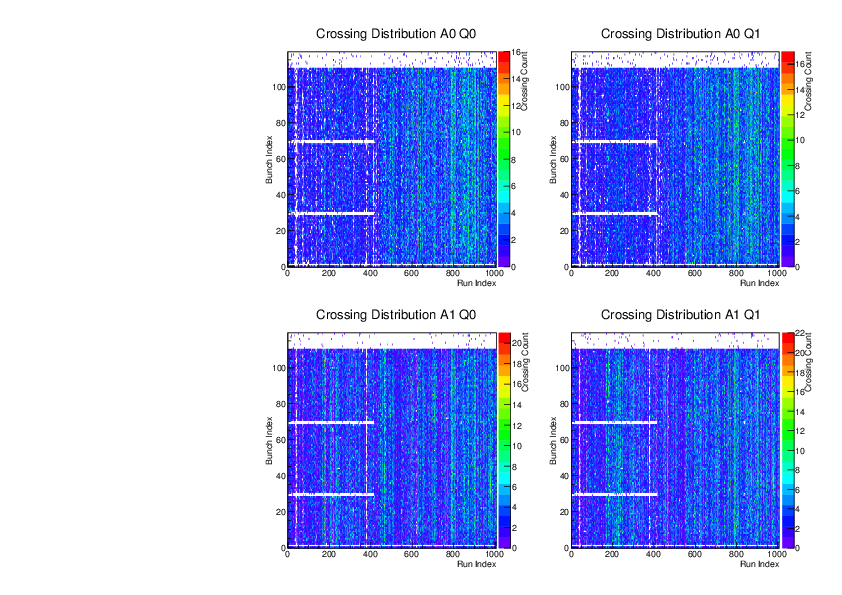
\includegraphics[width=\linewidth]{./figures/crossing_distribution.jpg}
  \caption{
    Shown: the crossing distribution for every run taken for the 2013 data
    set. We use the typical code for arm/charge. The top row is for the South
    Arm. The bottom row is for the North Arm. The left column is for negative
    charge, the right column is for positive charge. Note the characteristic
    empty abort gap, as well as the change from 109$\times$109 colliding bunches
    to 111$\times$111 colliding bunches about 1/3 of the way through the data
    taking period.
  }
  \label{fig:crossing_count}
\end{figure}

\begin{figure}
  \centering
  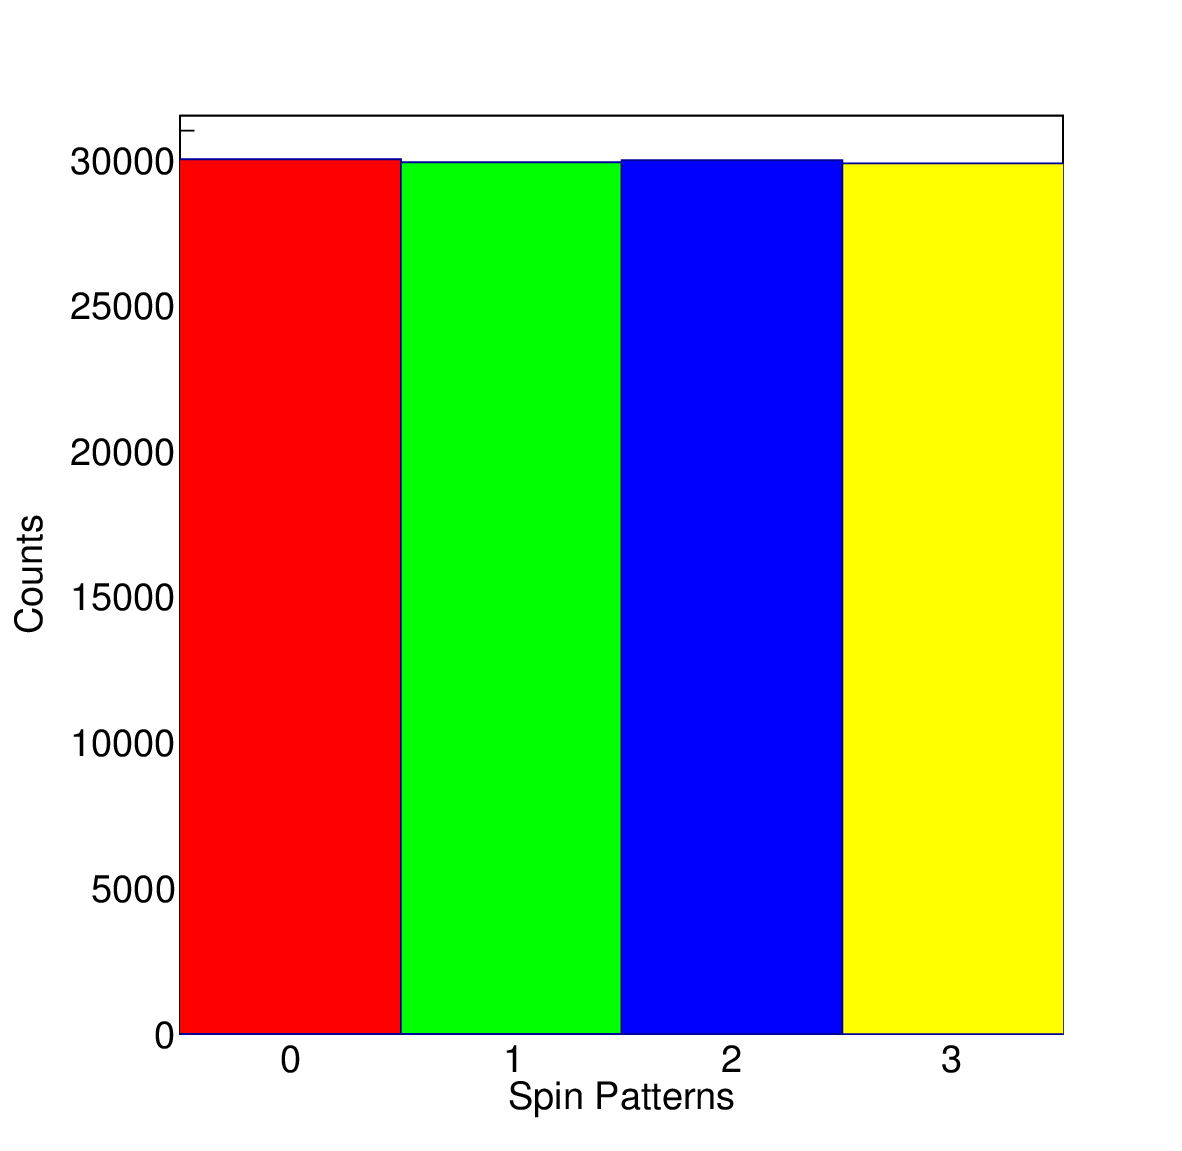
\includegraphics[width=0.6\linewidth]{./figures/crossing_pattenr_count.jpg}
  \caption{
    Shown: the yield for various crossing combinations as taken from
    the dataset itself, rather than the database. We see a very consistent
    distribution between the various possible crossing patterns. In this case,
    the horizontal axis is the crossing pattern code--0:$++$, 1:$-+$, 2:$+-$,
    3:$--$. Any slight difference between yields for each pattern is well below
    our experimental precision.
  }
  \label{fig:polarization_counts}
\end{figure}

With consistent distributions of polarization seen for each arm/charge, one does
not need to consider possible dilution of the asymmetry due to incorrect
accounting for polarization. Even so, this check has been done, and is presented
in the appendix. 

\clearpage
\section{Muon Yields}

Calculating $A_L$ requires obtaining yields for positive and negative rapidity
muons for all arm and charge conditions associated with the $W\rightarrow\mu$
signal process. 

Yields are obtained in the signal region by applying the $W_{ness}$ cut to the
recorded data set (cut events with $W_{ness} < 0.99 $), sorted into arm, charge,
and pseudorapidity bin. Each yield is then corrected for the signal to
background ratio, obtained from Section~\ref{sec:sbr}. The final muon yields are
summarized in Table~\ref{tab:south_sorted_muons_eta_bins} (south arm, three eta
bins), and Table~\ref{tab:north_sorted_muons_eta_bins} (north arm, three eta
bins).

Though there was enough integrated luminosity to separate data into six total
eta bins over the full rapidity range of the PHENIX muon arms, as a consistency
check to previous analysis which only had enough statistics for two $\eta$ bins,
one forward, and one backward for $A_L^{W+}$, I have also included data matching
previous binning, Table~\ref{tab:sorted_muons_standard}.

\begin{figure}
  \begin{minipage}[c]{0.67\textwidth}
    \centering
    \begin{tabular}{cccc}
      \toprule
      \multicolumn{4}{c}{\textbf{South Arm}} \\ 
      \textbf{Charge} & 
      \textbf{Helicity} & 
      \textbf{$\vert\eta\vert$ Range} &
      \textbf{$\mu$ Yield} \\ 
      \midrule
      $-1$ &\textbf{\textcolor{blue}{$+$}\textcolor{ucrgold}{$+$}} & $1.1 <\vert\eta\vert< 1.4$ & 12 \\
      $-1$ &\textbf{\textcolor{blue}{$+$}\textcolor{ucrgold}{$+$}} & $1.4 <\vert\eta\vert< 1.8$ & 67 \\
      $-1$ &\textbf{\textcolor{blue}{$+$}\textcolor{ucrgold}{$+$}} & $1.8 <\vert\eta\vert< 2.6$ & 63 \\
      $-1$ &\textbf{\textcolor{blue}{$-$}\textcolor{ucrgold}{$+$}} & $1.1 <\vert\eta\vert< 1.4$ & 21 \\
      $-1$ &\textbf{\textcolor{blue}{$-$}\textcolor{ucrgold}{$+$}} & $1.4 <\vert\eta\vert< 1.8$ & 99 \\
      $-1$ &\textbf{\textcolor{blue}{$-$}\textcolor{ucrgold}{$+$}} & $1.8 <\vert\eta\vert< 2.6$ & 49 \\
      $-1$ &\textbf{\textcolor{blue}{$+$}\textcolor{ucrgold}{$-$}} & $1.1 <\vert\eta\vert< 1.4$ & 19 \\
      $-1$ &\textbf{\textcolor{blue}{$+$}\textcolor{ucrgold}{$-$}} & $1.4 <\vert\eta\vert< 1.8$ & 76 \\
      $-1$ &\textbf{\textcolor{blue}{$+$}\textcolor{ucrgold}{$-$}} & $1.8 <\vert\eta\vert< 2.6$ & 58 \\
      $-1$ &\textbf{\textcolor{blue}{$-$}\textcolor{ucrgold}{$-$}} & $1.1 <\vert\eta\vert< 1.4$ & 14 \\
      $-1$ &\textbf{\textcolor{blue}{$-$}\textcolor{ucrgold}{$-$}} & $1.4 <\vert\eta\vert< 1.8$ & 68 \\
      $-1$ &\textbf{\textcolor{blue}{$-$}\textcolor{ucrgold}{$-$}} & $1.8 <\vert\eta\vert< 2.6$ & 57 \\
      $-1$ &\textbf{\textcolor{blue}{$*$}\textcolor{ucrgold}{$*$}} & $1.1 <\vert\eta\vert< 1.4$ & 0 \\
      $-1$ &\textbf{\textcolor{blue}{$*$}\textcolor{ucrgold}{$*$}} & $1.4 <\vert\eta\vert< 1.8$ & 0 \\
      $-1$ &\textbf{\textcolor{blue}{$*$}\textcolor{ucrgold}{$*$}} & $1.8 <\vert\eta\vert< 2.6$ & 0 \\
      $+1$ &\textbf{\textcolor{blue}{$+$}\textcolor{ucrgold}{$+$}} & $1.1 <\vert\eta\vert< 1.4$ & 28 \\
      $+1$ &\textbf{\textcolor{blue}{$+$}\textcolor{ucrgold}{$+$}} & $1.4 <\vert\eta\vert< 1.8$ & 94 \\
      $+1$ &\textbf{\textcolor{blue}{$+$}\textcolor{ucrgold}{$+$}} & $1.8 <\vert\eta\vert< 2.6$ & 50 \\
      $+1$ &\textbf{\textcolor{blue}{$-$}\textcolor{ucrgold}{$+$}} & $1.1 <\vert\eta\vert< 1.4$ & 26 \\
      $+1$ &\textbf{\textcolor{blue}{$-$}\textcolor{ucrgold}{$+$}} & $1.4 <\vert\eta\vert< 1.8$ & 96 \\
      $+1$ &\textbf{\textcolor{blue}{$-$}\textcolor{ucrgold}{$+$}} & $1.8 <\vert\eta\vert< 2.6$ & 41 \\
      $+1$ &\textbf{\textcolor{blue}{$+$}\textcolor{ucrgold}{$-$}} & $1.1 <\vert\eta\vert< 1.4$ & 22 \\
      $+1$ &\textbf{\textcolor{blue}{$+$}\textcolor{ucrgold}{$-$}} & $1.4 <\vert\eta\vert< 1.8$ & 124 \\
      $+1$ &\textbf{\textcolor{blue}{$+$}\textcolor{ucrgold}{$-$}} & $1.8 <\vert\eta\vert< 2.6$ & 47 \\
      $+1$ &\textbf{\textcolor{blue}{$-$}\textcolor{ucrgold}{$-$}} & $1.1 <\vert\eta\vert< 1.4$ & 26 \\
      $+1$ &\textbf{\textcolor{blue}{$-$}\textcolor{ucrgold}{$-$}} & $1.4 <\vert\eta\vert< 1.8$ & 97 \\
      $+1$ &\textbf{\textcolor{blue}{$-$}\textcolor{ucrgold}{$-$}} & $1.8 <\vert\eta\vert< 2.6$ & 66 \\
      $+1$ &\textbf{\textcolor{blue}{$*$}\textcolor{ucrgold}{$*$}} & $1.1 <\vert\eta\vert< 1.4$ & 0 \\
      $+1$ &\textbf{\textcolor{blue}{$*$}\textcolor{ucrgold}{$*$}} & $1.4 <\vert\eta\vert< 1.8$ & 0 \\
      $+1$ &\textbf{\textcolor{blue}{$*$}\textcolor{ucrgold}{$*$}} & $1.8 <\vert\eta\vert< 2.6$ & 0 \\
      \bottomrule
    \end{tabular}
  \end{minipage}\hfill
  \begin{minipage}[c]{0.3\textwidth}
    \caption{
      Shown: the South arm's yields for each helicity combination of colliding
      protons, with the polarization of the blue beam and yellow beams color
      coded in column 2. These yields represent all muons observed in the signal
      region, and are a combination of signal and background muons. + represents
      positive helicity beam polarization relative to the blue beam's momentum,
      - represents negative helicity, with * representing an unfilled bunch.
    }
    \label{tab:south_sorted_muons_eta_bins}
  \end{minipage}
\end{figure}

\begin{figure}
  \begin{minipage}[c]{0.67\textwidth}
    \centering
    \begin{tabular}{cccc}
      \toprule
      \multicolumn{4}{c}{\textbf{North Arm}} \\ 
      \textbf{Charge} & 
      \textbf{Helicity} & 
      \textbf{$\vert\eta\vert$ Range} &
      \textbf{$\mu$ Yield} \\ 
      \midrule
      $-1$ &\textbf{\textcolor{blue}{$+$}\textcolor{ucrgold}{$+$}} & $1.1 < \vert\eta\vert < 1.4$ & 18 \\
      $-1$ &\textbf{\textcolor{blue}{$+$}\textcolor{ucrgold}{$+$}} & $1.4 < \vert\eta\vert < 1.8$ & 76 \\
      $-1$ &\textbf{\textcolor{blue}{$+$}\textcolor{ucrgold}{$+$}} & $1.8 < \vert\eta\vert < 2.6$ & 57 \\
      $-1$ &\textbf{\textcolor{blue}{$-$}\textcolor{ucrgold}{$+$}} & $1.1 < \vert\eta\vert < 1.4$ & 14 \\
      $-1$ &\textbf{\textcolor{blue}{$-$}\textcolor{ucrgold}{$+$}} & $1.4 < \vert\eta\vert < 1.8$ & 63 \\
      $-1$ &\textbf{\textcolor{blue}{$-$}\textcolor{ucrgold}{$+$}} & $1.8 < \vert\eta\vert < 2.6$ & 56 \\
      $-1$ &\textbf{\textcolor{blue}{$+$}\textcolor{ucrgold}{$-$}} & $1.1 < \vert\eta\vert < 1.4$ & 13 \\
      $-1$ &\textbf{\textcolor{blue}{$+$}\textcolor{ucrgold}{$-$}} & $1.4 < \vert\eta\vert < 1.8$ & 74 \\
      $-1$ &\textbf{\textcolor{blue}{$+$}\textcolor{ucrgold}{$-$}} & $1.8 < \vert\eta\vert < 2.6$ & 61 \\
      $-1$ &\textbf{\textcolor{blue}{$-$}\textcolor{ucrgold}{$-$}} & $1.1 < \vert\eta\vert < 1.4$ & 19 \\
      $-1$ &\textbf{\textcolor{blue}{$-$}\textcolor{ucrgold}{$-$}} & $1.4 < \vert\eta\vert < 1.8$ & 63 \\
      $-1$ &\textbf{\textcolor{blue}{$-$}\textcolor{ucrgold}{$-$}} & $1.8 < \vert\eta\vert < 2.6$ & 65 \\
      $-1$ &\textbf{\textcolor{blue}{$*$}\textcolor{ucrgold}{$*$}} & $1.1 < \vert\eta\vert < 1.4$ & 0 \\
      $-1$ &\textbf{\textcolor{blue}{$*$}\textcolor{ucrgold}{$*$}} & $1.4 < \vert\eta\vert < 1.8$ & 0 \\
      $-1$ &\textbf{\textcolor{blue}{$*$}\textcolor{ucrgold}{$*$}} & $1.8 < \vert\eta\vert < 2.6$ & 0 \\
      $+1$ &\textbf{\textcolor{blue}{$+$}\textcolor{ucrgold}{$+$}} & $1.1 < \vert\eta\vert < 1.4$ & 24 \\
      $+1$ &\textbf{\textcolor{blue}{$+$}\textcolor{ucrgold}{$+$}} & $1.4 < \vert\eta\vert < 1.8$ & 96 \\
      $+1$ &\textbf{\textcolor{blue}{$+$}\textcolor{ucrgold}{$+$}} & $1.8 < \vert\eta\vert < 2.6$ & 60 \\
      $+1$ &\textbf{\textcolor{blue}{$-$}\textcolor{ucrgold}{$+$}} & $1.1 < \vert\eta\vert < 1.4$ & 30 \\
      $+1$ &\textbf{\textcolor{blue}{$-$}\textcolor{ucrgold}{$+$}} & $1.4 < \vert\eta\vert < 1.8$ & 95 \\
      $+1$ &\textbf{\textcolor{blue}{$-$}\textcolor{ucrgold}{$+$}} & $1.8 < \vert\eta\vert < 2.6$ & 64 \\
      $+1$ &\textbf{\textcolor{blue}{$+$}\textcolor{ucrgold}{$-$}} & $1.1 < \vert\eta\vert < 1.4$ & 27 \\
      $+1$ &\textbf{\textcolor{blue}{$+$}\textcolor{ucrgold}{$-$}} & $1.4 < \vert\eta\vert < 1.8$ & 68 \\
      $+1$ &\textbf{\textcolor{blue}{$+$}\textcolor{ucrgold}{$-$}} & $1.8 < \vert\eta\vert < 2.6$ & 64 \\
      $+1$ &\textbf{\textcolor{blue}{$-$}\textcolor{ucrgold}{$-$}} & $1.1 < \vert\eta\vert < 1.4$ & 33 \\
      $+1$ &\textbf{\textcolor{blue}{$-$}\textcolor{ucrgold}{$-$}} & $1.4 < \vert\eta\vert < 1.8$ & 99 \\
      $+1$ &\textbf{\textcolor{blue}{$-$}\textcolor{ucrgold}{$-$}} & $1.8 < \vert\eta\vert < 2.6$ & 56 \\
      $+1$ &\textbf{\textcolor{blue}{$*$}\textcolor{ucrgold}{$*$}} & $1.1 < \vert\eta\vert < 1.4$ & 0 \\
      $+1$ &\textbf{\textcolor{blue}{$*$}\textcolor{ucrgold}{$*$}} & $1.4 < \vert\eta\vert < 1.8$ & 0 \\
      $+1$ &\textbf{\textcolor{blue}{$*$}\textcolor{ucrgold}{$*$}} & $1.8 < \vert\eta\vert < 2.6$ & 0 \\
      \bottomrule
    \end{tabular}
  \end{minipage}\hfill
  \begin{minipage}[c]{0.3\textwidth}
    \caption{
      Shown: the North arm's yields for each helicity combination of colliding
      protons, with the polarization of the blue beam and yellow beams color
      coded in column 2. These yields represent all muons observed in the signal
      region, and are a combination of signal and background muons. + represents
      positive helicity beam polarization relative to the blue beam's momentum,
      - represents negative helicity, with * representing an unfilled bunch.
    }
    \label{tab:north_sorted_muons_eta_bins}
  \end{minipage}
\end{figure}

\begin{table}
  \centering
  \begin{tabular}{cccc}
    \toprule
    \textbf{Arm} &
    \textbf{Charge} & 
    \textbf{Helicity} & 
    \textbf{$\mu$ Yield} \\ 
    \midrule
    S & $-1$ & \textbf{\textcolor{blue}{$+$}\textcolor{ucrgold}{$+$}}& 142 \\
    S & $-1$ & \textbf{\textcolor{blue}{$-$}\textcolor{ucrgold}{$+$}}& 169 \\
    S & $-1$ & \textbf{\textcolor{blue}{$+$}\textcolor{ucrgold}{$-$}}& 153 \\
    S & $-1$ & \textbf{\textcolor{blue}{$-$}\textcolor{ucrgold}{$-$}}& 139 \\
    S & $-1$ & \textbf{\textcolor{blue}{$*$}\textcolor{ucrgold}{$*$}}& 0 \\
    S & $+1$ & \textbf{\textcolor{blue}{$+$}\textcolor{ucrgold}{$+$}}& 172 \\
    S & $+1$ & \textbf{\textcolor{blue}{$-$}\textcolor{ucrgold}{$+$}}& 163 \\
    S & $+1$ & \textbf{\textcolor{blue}{$+$}\textcolor{ucrgold}{$-$}}& 193 \\
    S & $+1$ & \textbf{\textcolor{blue}{$-$}\textcolor{ucrgold}{$-$}}& 189 \\
    S & $+1$ & \textbf{\textcolor{blue}{$*$}\textcolor{ucrgold}{$*$}}& 0 \\
    N & $-1$ & \textbf{\textcolor{blue}{$+$}\textcolor{ucrgold}{$+$}}& 151 \\
    N & $-1$ & \textbf{\textcolor{blue}{$-$}\textcolor{ucrgold}{$+$}}& 133 \\
    N & $-1$ & \textbf{\textcolor{blue}{$+$}\textcolor{ucrgold}{$-$}}& 148 \\
    N & $-1$ & \textbf{\textcolor{blue}{$-$}\textcolor{ucrgold}{$-$}}& 147 \\
    N & $-1$ & \textbf{\textcolor{blue}{$*$}\textcolor{ucrgold}{$*$}}& 0 \\
    N & $+1$ & \textbf{\textcolor{blue}{$+$}\textcolor{ucrgold}{$+$}}& 180 \\
    N & $+1$ & \textbf{\textcolor{blue}{$-$}\textcolor{ucrgold}{$+$}}& 189 \\
    N & $+1$ & \textbf{\textcolor{blue}{$+$}\textcolor{ucrgold}{$-$}}& 159 \\
    N & $+1$ & \textbf{\textcolor{blue}{$-$}\textcolor{ucrgold}{$-$}}& 188 \\
    N & $+1$ & \textbf{\textcolor{blue}{$*$}\textcolor{ucrgold}{$*$}}& 0 \\
    \bottomrule
  \end{tabular}
  \caption{
    Shown: a division of the yields by arm, charge, and helicity combination,
    which is color-coded for the polarization of the blue and yellow beams.
    Yields contain a combination of signal and background muons. + represents
    positive helicity beam polarization relative to the blue beam's momentum, -
    represents negative helicity, with * representing an unfilled bunch.
  }
  \label{tab:sorted_muons_standard}
\end{table}

With the extraction of the yields and confirmation that the beam polarization is
well behaved, the asymmetries are calculated and corrected for the signal to
background dilution, and the beam polarization. Any non-vanishing asymmetry with
such corrections represents actual physical asymmetries.

\clearpage
\section{Calculation of $\epsilon_L$ and $A_{L}$ for $W\rightarrow\mu$}
\label{sec:calculate_al}

With an understanding of beam polarization and the signal to background ratio,
the asymmetries are calculated. One first proceeds the calculation of the raw
asymmetry, $\epsilon_L$, directly from the raw muon yields, and subsequently
corrects for dilution from background events and beam polarization to obtain the
true longitudinal asymmetry, $A_L$.

\subsection{Defining $A_L^{W\pm}$, $A_{LL}^{W\pm}$}

There is a lot of language and terminology inherited from previous work in Deep
Inelastic Scattering Experiments and the models developed to characterize the
results of these experiments. One such concept is the idea of a `probe'
particle, and a `target' particle. In DIS experiments, especially those designed
to study proton polarization, there is typically a high energy electron beam
impinging on a spin polarized gas target. Asymmetries were then defined in terms
of scattering cross sections, where the polarization of the beam (or probe) and
target were known.

For the case of RHIC, this formalism must be translated to describe an
intersecting ring collider. Since final state of the $W\rightarrow\mu$ is
measured, and the initial polarization state of the colliding protons is known,
one may adopt the formalism, assigning one proton to the `probe' and the other
to the `target'.  Our convention is to take the polarized proton as our target,
and then assume the other proton is our `probe', subsequently summing over the
various probe polarizations. In this way, the asymmetries are measured in $W$
boson production.

To describe the asymmetry intuitively: the longitudinal asymmetry for $W$ boson
production refers to the difference in $W$ Boson production for two different
initial-state proton polarizations.  Mathematically, this is formalized by
normalizing this total difference in production with the total production of $W$
Bosons from both polarization states. Because we may treat the blue beam as the
probe \textit{or} the target (similarly with the yellow beam), one must take
care, because the helicity of the initial state protons is defined as positive
or negative relative to the probe beam's momentum. Therefore, because PHENIX
records and labels data according to its coordinate system, the sign of
pseudorapidity might switch based on which beam is the probe, and which beam of
the target, when calculating asymmetries. This convention is summarized in
Table~\ref{tab:asymmetry_rapidity_convention}. The convention can be summarized
as ``when is a factor of -1 applied to the rapidity measured with respect to the
PHENIX coordinate system''.

\begin{table}[ht]
  \centering
  \begin{tabular}{ccccc}
    \toprule
    \textbf{Arm} & 
    \textbf{Charge} &
    \textbf{Probe Beam} & 
    \textbf{Target Beam} & 
    \textbf{Sign of $\eta$} \\
    \midrule
    N & $\mu^+$ & Blue   & Yellow & $+\eta$ \\
    N & $\mu^-$ & Blue   & Yellow & $+\eta$ \\
    S & $\mu^+$ & Blue   & Yellow & $-\eta$ \\
    S & $\mu^-$ & Blue   & Yellow & $-\eta$ \\
    N & $\mu^+$ & Yellow & Blue   & $-\eta$ \\
    N & $\mu^-$ & Yellow & Blue   & $-\eta$ \\
    S & $\mu^+$ & Yellow & Blue   & $+\eta$ \\
    S & $\mu^-$ & Yellow & Blue   & $+\eta$ \\
    \bottomrule
  \end{tabular}
  \caption{
    A summary of the sign convention when we consider rapidity with respect to
    the probe beam, as opposed to the rapidity of the PHENIX coordinate system.
    Column \textbf{Sign of $\eta$} refers to the sign of $\eta$ of the observed
    muon track with respect to the probe beam.
  }
  \label{tab:asymmetry_rapidity_convention}

\end{table}

It is very important to stick with our convention, as it allows us to combine
the results of the raw asymmetries, to obtain a full description for
$A_L^{W\pm}$, since $W^\pm$ may decay into forward, or backward rapidities.
Proceeding with the asymmetry calculation, with our conventions defined:

{\noindent}For any fixed rapidity bin, we write down the Single Spin Asymmetry,
for $W^\pm\rightarrow\mu$ production:

\begin{equation}
  A_L = {
    {d\sigma^{\Rightarrow}-d\sigma^{\Leftarrow}}
    \over
    {d\sigma^{\Rightarrow}+d\sigma^{\Leftarrow}}
  }
\end{equation}

{\noindent}Recall from earlier that $\Leftarrow$ refers to the negative helicity
condition of the probe proton, while $\Rightarrow$ refers to the negative
helicity positive helicity of the probe proton. The helicity states of the
target proton are summed over. The double spin asymmetry, $A_{LL}$, is defined
similarly:

\begin{equation}
  A_{LL} = {
    {d\sigma^{\Rightarrow\Rightarrow}-d\sigma^{\Leftarrow\Rightarrow}}
    \over
    {d\sigma^{\Rightarrow\Rightarrow}+d\sigma^{\Leftarrow\Rightarrow}}
  }
\end{equation}

$A_{LL}$ is calculated as a positivity constraint~\cite{Kang2011} in order
restrict the allowed domain for spin observables. $A_{LL}$ gives access to the
product of quark and anti-quark polarizations, which is an important systematic
effect which providing a constraint on the quark polarization. In this case the
helicity states of the probe and target proton are indicated with $\Rightarrow$
and $\Leftarrow$, with the left-hand arrow referring to the probe, and the
right-hand arrow referring to the target.

With the required elements ready to calculate our asymmetries, the muon yields,
beam polarization, the signal to background ratio, and the rapidity convention,
the asymmetries are calculated. 

{\noindent}Yields for the south arm are denoted:
\begin{equation}
  \left\{
  n_{\left(++\right)}^S,
  n_{\left(+-\right)}^S,
  n_{\left(-+\right)}^S,
  n_{\left(--\right)}^S
  \right\}
  \label{eq:muon_yield_south}
\end{equation}

{\noindent}and north arm:
\begin{equation}
  \left\{
  n_{\left(++\right)}^N,
  n_{\left(+-\right)}^N,
  n_{\left(-+\right)}^N,
  n_{\left(--\right)}^N
  \right\}
  \label{eq:muon_yield_north}
\end{equation}

With the $+$ and $-$ signs indicating the polarization of the beams, (left sign
refers to blue polarization, right sign refers to yellow polarization).
Implicitly, these yields are taken with respect to an $\eta$ bin.

\subsection{Calculating $A_L^{W\pm}$, $A_{LL}^{W\pm}$}
\label{sec:calculating_al}

The asymmetries are calculated:

\noindent\textbf{Single Spin Asymmetries}\\

\noindent\textbf{Polarized Blue Probe, Yellow Target, $\eta > 0$ w.r.t. Probe}
\begin{equation}
  {\epsilon_{L,N}^{\eta > 0}} 
  = 
  { 
    {\sigma^\Rightarrow-\sigma^\Leftarrow} 
    \over 
    {\sigma^\Rightarrow+\sigma^\Leftarrow} 
  } 
  \to 
  {
    {\left(n_{(++)}^N+n_{(+-)}^N\right)-\left(n_{(-+)}^N+n_{(--)}^N\right)}
    \over
    {\left(n_{(++)}^N+n_{(+-)}^N\right)+\left(n_{(-+)}^N+n_{(--)}^N\right)}
  }
  \label{eq:al_blue_probe_pos_rap}
\end{equation}\\

\noindent\textbf{Polarized Blue Probe, Yellow Target, $\eta < 0$ w.r.t Probe}
\begin{equation}
  {\epsilon_{L,S}^{\eta < 0}} 
  = 
  { 
    {\sigma^\Rightarrow - \sigma^\Leftarrow} 
    \over 
    {\sigma^\Rightarrow + \sigma^\Leftarrow} 
  } 
  \to 
  {
    {\left(n_{(++)}^S+n_{(+-)}^S\right)-\left(n_{(-+)}^S+n_{(--)}^S\right)}
    \over
    {\left(n_{(++)}^S+n_{(+-)}^S\right)+\left(n_{(-+)}^S+n_{(--)}^S\right)}
  }
  \label{eq:al_blue_probe_neg_rap}
\end{equation}\\

\noindent\textbf{Polarized Yellow Probe, Blue Target, $\eta > 0$ w.r.t Probe}
\begin{equation}
  {\epsilon_{L,S}^{\eta > 0}} 
  = 
  { 
    {\sigma^\Rightarrow-\sigma^\Leftarrow} 
    \over 
    {\sigma^\Rightarrow+\sigma^\Leftarrow} 
  } 
  \to 
  {
    {\left(n_{(++)}^S+n_{(-+)}^S\right)-\left(n_{(+-)}^S+n_{(--)}^S\right)}
    \over
    {\left(n_{(++)}^S+n_{(-+)}^S\right)+\left(n_{(+-)}^S+n_{(--)}^S\right)}
  }
  \label{eq:al_yell_probe_pos_rap}
\end{equation}\\

\noindent\textbf{Polarized Yellow Probe, Blue Target, $\eta < 0$ w.r.t Probe}
\begin{equation}
  {\epsilon_{L,N}^{\eta < 0}} 
  = 
  { 
    {\sigma^\Rightarrow-\sigma^\Leftarrow} 
    \over 
    {\sigma^\Rightarrow+\sigma^\Leftarrow} 
  } 
  \to 
  {
    {\left(n_{(++)}^N+n_{(-+)}^N\right)-\left(n_{(+-)}^N+n_{(--)}^N\right)}
    \over
    {\left(n_{(++)}^N+n_{(-+)}^N\right)+\left(n_{(+-)}^N+n_{(--)}^N\right)}
  }
  \label{eq:al_yell_probe_neg_rap}
\end{equation}\\

\noindent\textbf{Double Spin Asymmetries} \\

\noindent\textbf{$A_{LL}$ North Arm}
\begin{equation}
  {\epsilon_{LL,N}}
  = 
  { 
    {\sigma^{\Rightarrow\Rightarrow}-\sigma^{\Leftarrow\Rightarrow}} 
    \over 
    {\sigma^{\Rightarrow\Rightarrow}+\sigma^{\Leftarrow\Rightarrow}} 
  } 
  \to 
  {
    {\left(n_{(++)}^N+n_{(--)}^N\right)-\left(n_{(+-)}^N+n_{(-+)}^N\right)}
    \over
    {\left(n_{(++)}^N+n_{(--)}^N\right)+\left(n_{(+-)}^N+n_{(-+)}^N\right)}
  }
  \label{eq:all_north}
\end{equation}\\

\noindent\textbf{$A_{LL}$ South Arm}
\begin{equation}
  {\epsilon_{LL,S}}
  = 
  { 
    {\sigma^{\Rightarrow\Rightarrow}-\sigma^{\Leftarrow\Rightarrow}} 
    \over 
    {\sigma^{\Rightarrow\Rightarrow}+\sigma^{\Leftarrow\Rightarrow}} 
  } 
  \to 
  {
    {\left(n_{(++)}^S+n_{(--)}^S\right)-\left(n_{(+-)}^S+n_{(-+)}^S\right)}
    \over
    {\left(n_{(++)}^S+n_{(--)}^S\right)+\left(n_{(+-)}^S+n_{(-+)}^S\right)}
  }
  \label{eq:all_south}
\end{equation}\\

In all cases, $\epsilon$ refers to the raw asymmetry, i.e. an asymmetry which
has not been corrected for dilution due to background contamination of the
yields, or dilution due to less than 100\% beam polarization.

{\noindent}The correction for either dilution is straight-forward:

\begin{gather}
  {A_L^{\eta>0}} = {{D^N}\over{P_B}}{\epsilon_{L,N}^{\eta>0}} = {{D^S}\over{P_Y}}{\epsilon_{L,S}^{\eta>0}} \\
  {A_L^{\eta<0}} = {{D^N}\over{P_B}}{\epsilon_{L,N}^{\eta<0}} = {{D^S}\over{P_Y}}{\epsilon_{L,S}^{\eta<0}} \\
  {A_{LL}}       = {{D^N}\over{P_BP_Y}}{\epsilon_{LL,N}}      = {{D^S}\over{P_BP_Y}}{\epsilon_{LL,S}}       
  \label{eq:dilution_correction}
\end{gather}

\subsection{Preliminary Results}

My analysis group earned PHENIX preliminary status for these results in October
of 2015.  The results were submitted for collaboration review,
and were judged worthy of showing at conferences 

The calculated asymmetries are shown in three $\eta$ bins per arm in
Figure~\ref{fig:al_preliminary_three_eta}. The asymmetries calculated for
comparison with the previous $\eta$ binning contention are shown in
Figure~\ref{fig:al_preliminary_standard}. The signal to background ratios and
yields were calculated from the signal region, $W_{ness} > 0.99$. 

\begin{figure}[ht]
  \centering
  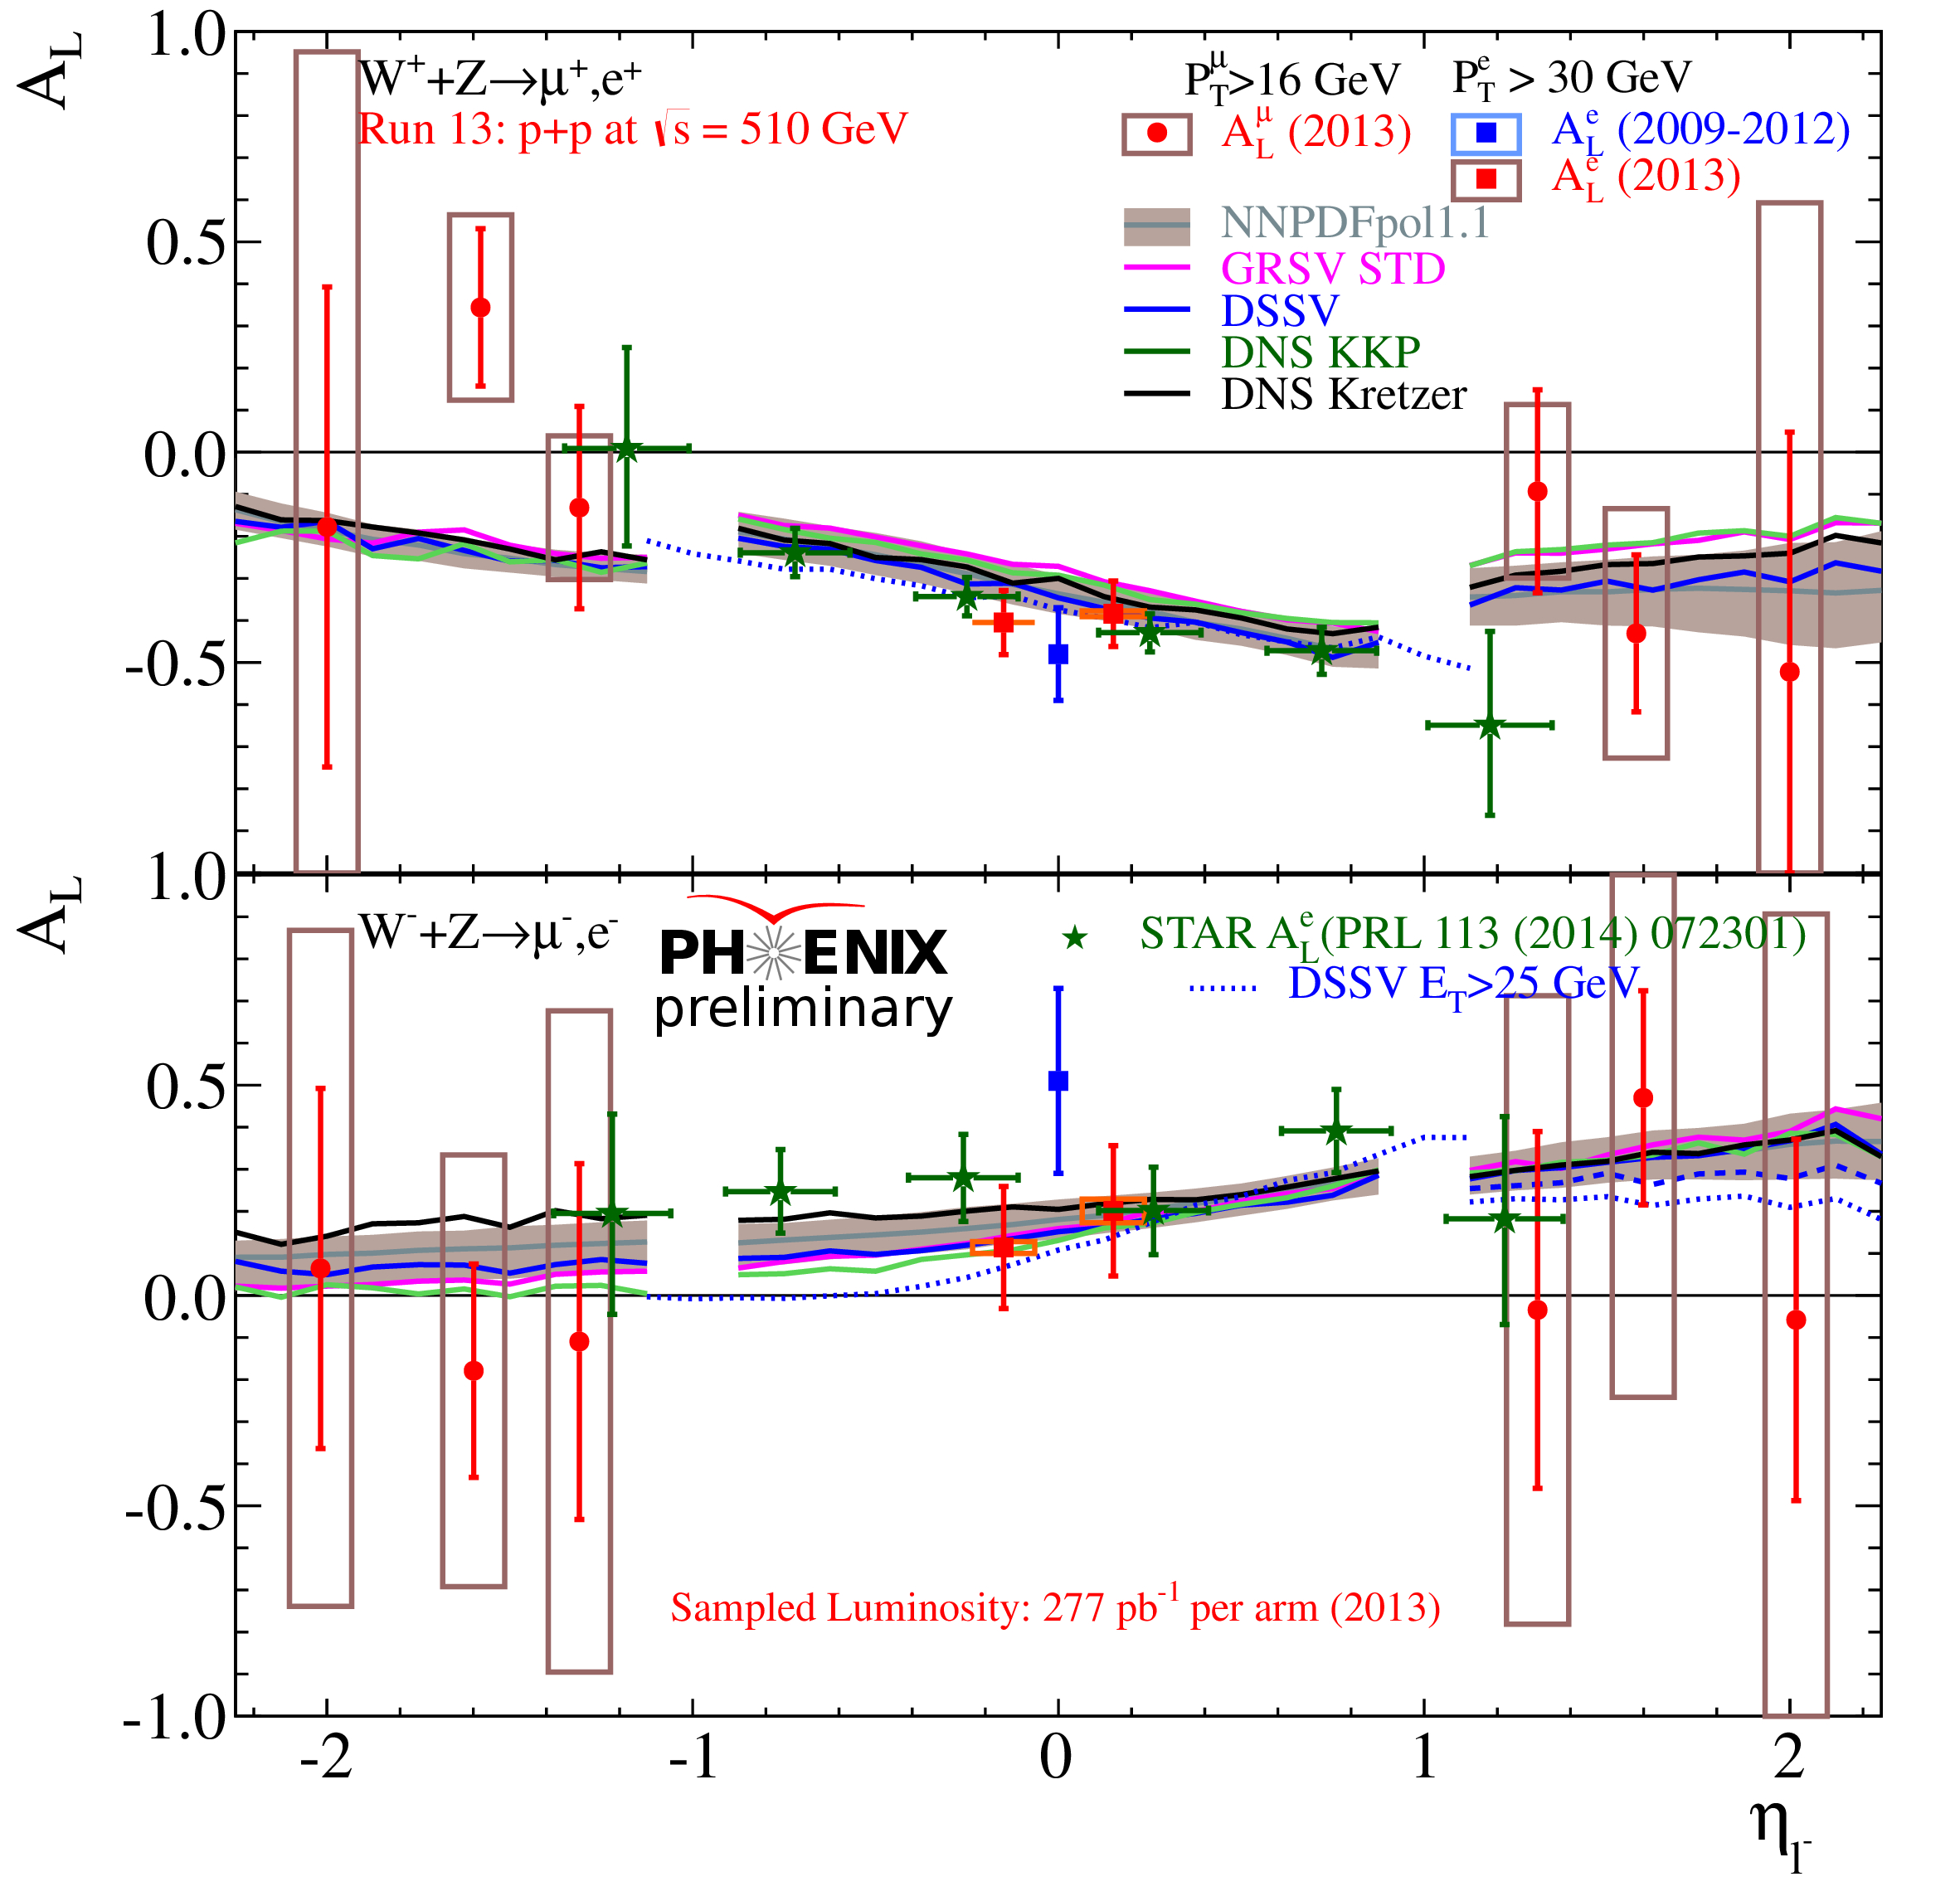
\includegraphics[width=0.8\linewidth]{./figures/prelim_AL_6bins.jpg}
  \caption{
    Shown: the preliminary longitudinal single spin asymmetries for three
    distinct bins in $\eta$ per Muon Arm. The red boxed points represent the
    measured asymmetry from the 2013 analysis. The green points show the central
    rapidity asymmetries produced from STAR in 2014, with the blue points
    showing PHENIX's central asymmetries from 2009-2012. The colored curves are
    superimposed predicted asymmetries. The top panel shows results for the
    $W^+$ process, with the bottom panel showing results for the $W^-$ process.
  }
  \label{fig:al_preliminary_three_eta}
\end{figure}

\begin{figure}[ht]
  \centering
  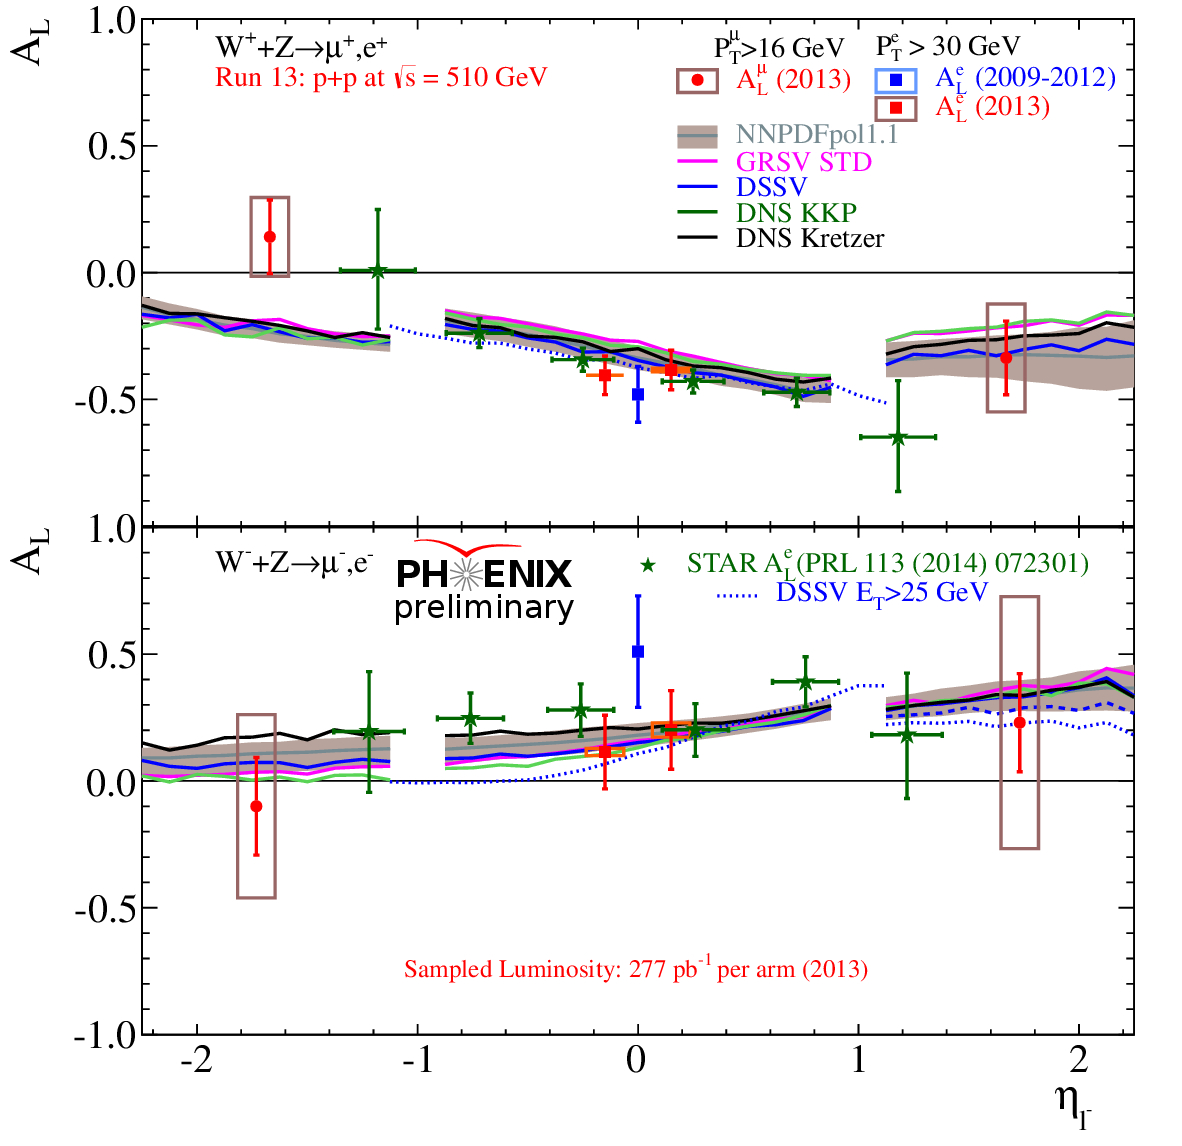
\includegraphics[width=0.8\linewidth]{./figures/prelim_AL_2bins.jpg}
  \caption{
    Shown: the preliminary longitudinal single spin asymmetries for two distinct
    bins in $\eta$ per Muon Arm. The red boxed points represent the measured
    asymmetry from the 2013 analysis. The green points show the central rapidity
    asymmetries produced from STAR in 2014, with the blue points showing
    PHENIX's central asymmetries from 2009-2012. The colored curves are
    superimposed predicted asymmetries. The top panel shows results for the
    $W^+$ process, with the bottom panel showing results for the $W^-$ process.
  }
  \label{fig:al_preliminary_standard}
\end{figure}
